\chapter{Crypto.Symmetric.Mode}\label{Mode}
With this package it is possible to work with a block cipher in a
secure operating mode. Generally an operating mode integrates a block
cipher with a feedback and some easy operations ($+,xor$), and will be
initialized with a random start value (IV). Thus the ciphertext
depends not only on plaintext and key, but also on the random start
value. If man encrypts twice a plaintext with the same cipher key but
different IVs, then man gets different ciphertexts. With the feedback
that two same plaintext blocks will be encrypted to different
ciphertext blocks, i.e. in an operating mode two plaintext blocks
$P_1$ and $P_2$ with $P_1=P_2$ are encrypted, with absolute
probability to two ciphertext blocks $C_1$ and $C_2$ with $C_1\neq
C_2$. For this reason it is now possible to encrypt more messages
securely under the same key.\\

\noindent\textbf{Remark: To decrypt a ciphertext, man needs the same
  key and IV which used in encryption.}  One should always keep the IV
with the related ciphertext. \textbf{The security of a mode is
  independent on the familarity of the start value.} Therefore it is
in general, that man concatenates the ciphertext to the end of the
start value to get the final output $C'$ ($C'=IV||C$). In this chapter
several kinds of modes will be introduced.

%%%%%%%%%%%%%%%%%%%%%%%%%%%%%%%%%%%%%%%%%%%%%%%%%%%%%%%%

\section{API}\label{API-Mode}
The API of a mode is made of four procedures.
\begin{itemize}
\item One procedure \texttt{Init()}; it initializes a mode by
  assigning a key and an initial value.
\begin{lstlisting}{}
  procedure Init(Key : in Key_Type; Initial_Value : in Block);
\end{lstlisting}
\item One procedure \texttt{Encrypt()};
\begin{lstlisting}{}
  procedure Encrypt(Plaintext: in Block; Ciphertext: out Block);
\end{lstlisting}
\item One procedure \texttt{Decrypt()};
\begin{lstlisting}{}
  procedure Decrypt(Ciphertext: in Block; Plaintext: out Block);
\end{lstlisting}
\item One procedure \texttt{Set\_IV()}; it assigns the start
  value. The mode should be reinitialized after every encryption or
  decryption (A message is made of $n$ plaintext blocks, which
  corresponds with $n$ calls of the \texttt{Encrypt()} or
  \texttt{Decrypt()} procedures).
\begin{lstlisting}{}
  procedure Set_IV(Initial_Value : in Block);
\end{lstlisting}
\end{itemize}

%%%%%%%%%%%%%%%%%%%%%%%%%%%%%%%%%%%%%%%%%%%%%%%%%%%%%%%%%
%%%%%%%%%%%%%%%%%%%%%%%%%%%%%%%%%%%%%%%%%%%%%%%%%%%%%%%%%

\section{Cipher Block Chaining Mode (CBC)}
\subsubsection*{Package: Crypto.Symmetric.Mode.CBC}
In the CBC mode, each block of plaintext will be XORed with the
previous ciphertext block before being encrypted (for the first time
XORed with an initial value). This way, each outputed ciphertext block
depends on all plaintext blocks processed up to that point
\cite{DBLP:reference/crypt/2011}.
\subsubsection*{Encryption}
Mathematical description: $C_i=E_K(P_i\oplus C_{i-1})\,, C_0=IV$\,.

Figure \ref{CBCEN} shows the workflow of the CBC encryption.  By the
initialization, the start value IV will be stored as $C_0$. A
plaintext block $P_1$ is to encrypt, it will be XORed with $C_0$ and
then encrypted to a ciphertext block $C_1$. The next plaintext block
$P_2$ will XORed with $C_1$ and then encrypted to $C_2$ and so on.
\begin{figure}[h]
\centering
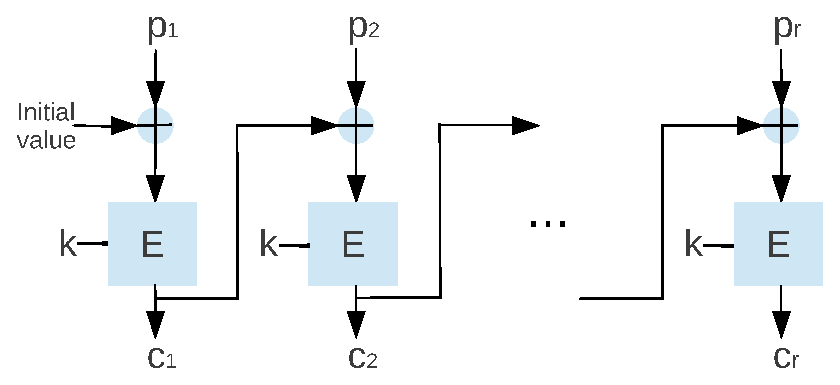
\includegraphics[scale=0.8]{./images/CBC_En}
\caption{Workflow of the CBC encryption. Adapted from
  \cite{DBLP:reference/crypt/2011}.}\label{CBCEN}
\end{figure}
\subsubsection*{Decryption}
Mathematical description: $P_i=C_{i-1}\oplus D_K(C_i)$.

Figure \ref{CBCDE} shows the decryption workflow of CBC. It's the
reverse of encryption. At the beginning the mode will be initialized
with IV or in \texttt{Set\_IV()} reinitialized. A ciphertext block
$C_1$ will be decrypted and the output will be XORed with $C_0$. The
result of the XOR operation is the plaintext block $P_1$. The next
ciphertext block $C_2$ will be decrypted and the output will be XORed
with $C_1$ as $P_2$ and so on.
\begin{figure}[h]
\centering
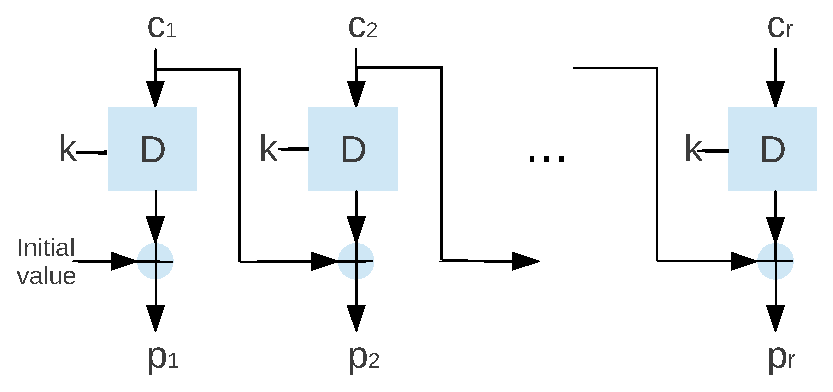
\includegraphics[scale=0.8]{./images/CBC_De}
\caption{Workflow of the CBC decryption. Adapted from
  \cite{DBLP:reference/crypt/2011}.}\label{CBCDE}
\end{figure}
\subsubsection*{Purpose of Use}
\begin{itemize}
\item \textbf{Data Encryption}\\ Since there can be no error by
  synchronization in this mode, it is useful for data
  encryption. However it can lead to bit errors (through defective
  hardware or the like). One bit error in a ciphertext block $C_i$ can
  influence the plaintext block $P_i$ and also the related bit in next
  plaintext block $P_{i+1}$.
\item \textbf{Message Integrity Testing}\\ In order to test the
  integrity of a message, we encrypt the message and only need to
  remember two ciphertext blocks: $C_0=IV$ and $C_n$. The remaining
  ciphertext blocks are not required. Now we can certify at any time
  by encrypting the message $M$ to $C'_n$ with the start value $C_0$
  and compare $C_n$ with $C'_n$, whether the message is changed or
  not. If $C_n=C'_n$, then the message $M$ is the original one,
  otherweise at least one of $IV$, $C_n$ or $M$ is changed. "Changed"
  is understood as accidental tipping of one or more bits.
\item \textbf{Message Authenticity Testing}\\ Supposed that you tell
  Alice a key, who you'd never met before. And one day you want to
  meet Alice to exchange secret data. To ensure that the people at the
  meeting point is really Alice, you bring a message $M$ and a
  randomly start value $IV$. You ask Alice to encrypt the message to
  $C'_n$ with the key and the start value. If $C'_n$ agrees with your
  computed $C_n$ (neither you nor Alice has told anyone the key), then
  the person is with significant propability to be Alice. If the two
  values are not the same, then the person is not Alice.
\item \textbf{Notice: The CBC-Mode is only secure when the exchanged
  messages are at the same length.} So users should pay attention to
  use the CBC Mode.
\end{itemize}

%%%%%%%%%%%%%%%%%%%%%%%%%%%%%%%%%%%%%%%%%%%%%%%%%%%%%%%%%
%%%%%%%%%%%%%%%%%%%%%%%%%%%%%%%%%%%%%%%%%%%%%%%%%%%%%%%%%

\section{BPS}
\subsubsection*{Package: Crypto.Symmetric.Mode.BPS}
BPS is a generic format-preserving symmetric encryption algorithm,
which can cipher short or long string of characters from any given
set, e.g. credit card numbers.

\subsubsection*{Encryption and Decryption}
The main process is similar to the CBC mode with an IV set to 0.
Internally a 8-round encryption is used. The plaintext will be divided
into two sub-strings $L,R$ of similar length, i.e. $P=L||R$, and each
of them will be updated in turn \cite{BPS}. Decryption is also
composed of 8 rounds. They work as shown in Figure \ref{BPSED}.
\begin{figure}[htp]
\center
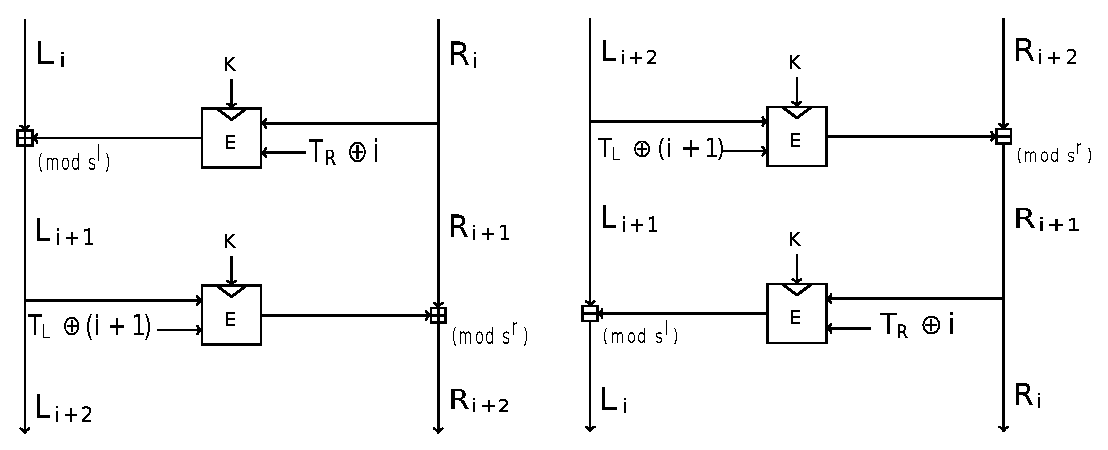
\includegraphics[scale=0.8]{./images/BPS_En_De}
\caption{Workflow of the internal encryption (Left) and decryption
  (Right) in the BPS. \cite{BPS}}\label{BPSED} \center
\end{figure}


\noindent\textbf{Remarks}
\begin{itemize}
\item One advantage of BPS is its adaptability, all the block cipher
  and hash function standardized primitives (TDES, AES or SHA-2) can
  be used as basic internal bricks \cite{BPS}.
\item The internal tweak values is useful to avoid some kind of
  dictionary attacks \cite{BPS}. Indeed, if no tweak is used, a third
  party could build a dictionary of plaintext / ciphertext pairs and
  find with good probability the eavesdropped encrypted PANs (Personal
  Account Numbers), this attack works when the amount of data is
  small, which is particularly the case for an array of numbers
  encryption \cite{BPS}. "Using random tweak will render this
  dictionary technique useless as one dictionary per tweak value would
  be required" \cite{BPS}.
\item An essential quality of BPS is its efficiency. Due to that the
  input key for all the block cipher internal calls is constant, this
  requires only one internal cipher key per BPS encryption, which
  saves a lot of operations and time \cite{BPS}. Moreover, w = 8
  rounds is recommanded, it makes the whole encryption process very
  efficient \cite{BPS}.
\end{itemize}
%%%%%%%%%%%%%%%%%%%%%%%%%%%%%%%%%%%%%%%%%%%%%%%%%%%%%%%%%
%%%%%%%%%%%%%%%%%%%%%%%%%%%%%%%%%%%%%%%%%%%%%%%%%%%%%%%%%
\section{Cipher Feedback Mode (CFB)}\label{CipherFeedbackMode}
\subsubsection*{Package: Crypto.Symmetric.Mode.CFB}
The cipher feedback (CFB) mode, a close relative of CBC, makes a block
cipher into a self-synchronizing stream cipher
\cite{DBLP:reference/crypt/2011}.
\begin{figure}[htp]
\center
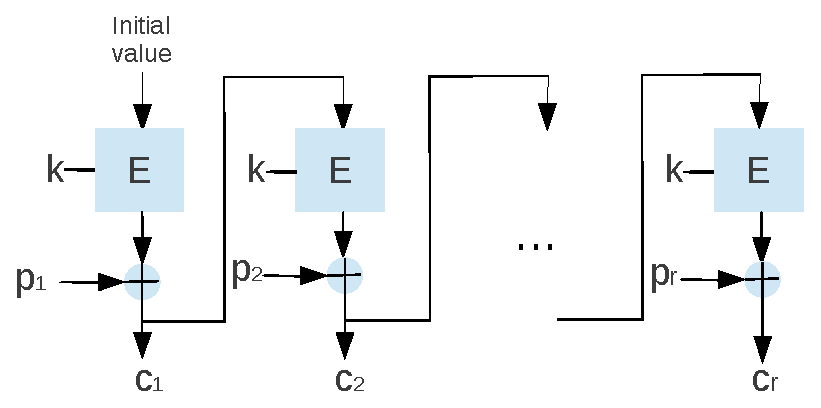
\includegraphics[scale=0.8]{./images/CFB_En}
\caption{Workflow of the CFB encryption. Adapted from
  \cite{DBLP:reference/crypt/2011}.}\label{CFBEN} \center
\end{figure}

\subsubsection*{Encryption}
Mathematical description : $C_i=E_K(C_{i-1})\oplus P_i$,
$C_0=IV$.

Figure \ref{CFBEN} shows the workflow of encryption in CFB. By
initialization the start value IV will be stored as $C_0$. To encrypt
a $n$ bit ($n<$ Block'Size) message, it will be copied in the
plaintext block, and then padded with zeros. To encrypt a plaintext
block $P_1$, the start value $C_0$ will be encrypted at first, and
then XORed with $P_1$ and stored as $C_1$. Following plaintext blocks
will be processed iteratively until the complete message is encrypted.

\subsubsection*{Decryption}
Mathematical description : $P_i=E_K(C_{i-1})\oplus C_i$,
$C_0=IV$.

As shown in Figure \ref{CFBDE}, the decryption in CFB makes use of the
encryption algorithm. At the beginning the mode will be initialized or
through \texttt{Set\_IV()} reinitialized. To decrypt a ciphertext
block $C_i$, $C_{i-1}$ will be decrypted at first and then XORed with
$C_i$. The output of the operation is $P_i$.
\begin{figure}[h]
\centering
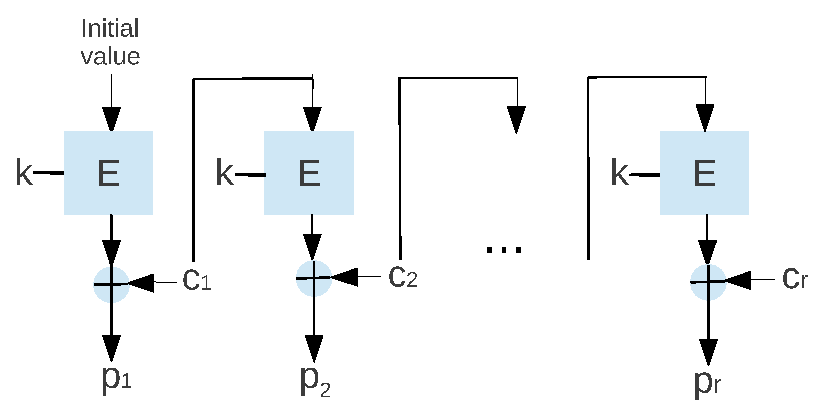
\includegraphics[scale=0.8]{./images/CFB_De}
\caption{Workflow of the CFB decryption. Adapted from
  \cite{DBLP:reference/crypt/2011}.} \label{CFBDE}
\end{figure}
\subsubsection*{Remarks}
In comparison with CBC-Mode, which can be used when a complete data
block exists, CFB-Mode can be used to encrypt not only data but also
bytes (8-CFB). Therefore it is mainly used for encryption of byte
streams (e.g. Remote shell).

 In n-CFB-Mode:
\begin{itemize}
\item an error in plaintext will affect the following complete
  ciphertext and in decryption it goes backward.
\item an error in ciphertext $C_i$ will affect the plaintext block
  $P_i$ and also the following $\frac{m}{n}-1$ plaintext blocks, where
  $m$ is the size of the message.
\item An aggressor can change the message bits in the last ciphertext
  block without being found.
\end{itemize}

%%%%%%%%%%%%%%%%%%%%%%%%%%%%%%%%%%%%%%%%%%%%%%%%%%%%%%%%%
%%%%%%%%%%%%%%%%%%%%%%%%%%%%%%%%%%%%%%%%%%%%%%%%%%%%%%%%%

\section{Counter Mode (CTR)}\label{CounterMode}
\subsubsection*{Package: Crypto.Symmetric.Mode.CTR}
In Counter Mode the feedback isn't dependent on plaintext, but on a
counter, which will be increased by 1 after every encryption. Note
that the nonce in Figure \ref{CTREN} and Figure \ref{CTRDE} is the
same thing as the initial vector (IV) in other graphs.

\subsubsection*{Encryption}
Mathematical description : $C_i=P_i\oplus E_K(IV+i-1)$.\\ In Figure
\ref{CTREN} the counter is initialized at first. The current counter
$IV+i-1$ of each block is encrypted, the output is then XORed with
plaintext block $P_i$, and the result is $C_i$.
\begin{figure}[h]
\centering
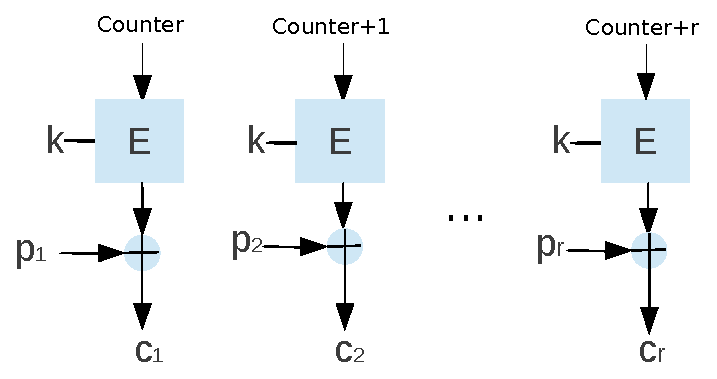
\includegraphics[scale=0.8]{./images/CTR_En}
\caption{Workflow of the CTR encryption. Adapted from
  \cite{DBLP:reference/crypt/2011}.}\label{CTREN}
\end{figure}
\subsubsection*{Decryption}
Mathematical description : $P_i=C_i\oplus E_K(IV+i-1)$.

Note that in Figure \ref{CTRDE} the encryption algorithm is used in
decryption.  After initialization counter $IV+i-1$ will be encrypted,
then the output will be XORed with $C_i$ and the result is $P_i$. It
is done iteratively until the last block.
\begin{figure}[h]
\centering
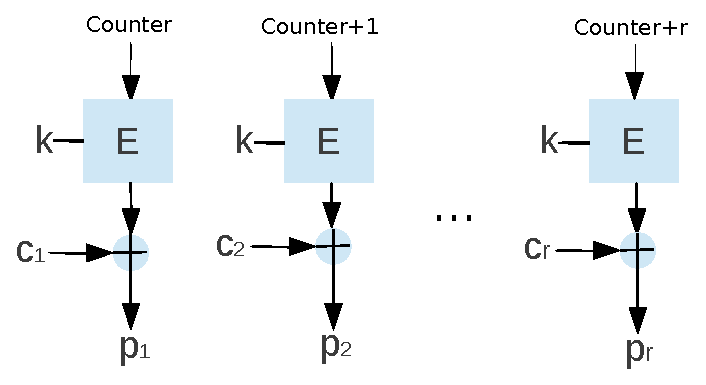
\includegraphics[scale=0.8]{./images/CTR_De}
\caption{Workflow of the CTR decryption. Adapted from
  \cite{DBLP:reference/crypt/2011}.}\label{CTRDE}
\end{figure}
\subsubsection*{Remarks}
\begin{itemize}
\item \textbf{En-/Decryption of Messages with Random Access}\\
Since that the counter mode is used to decrypt individual ciphertext
block, this procedure is suitable for decryption of data with random
access e.g. Database.
\item \textbf{Parallel En-/Decryption}\\
Parallelization is possible when man calculates an interval from the
start value (IV) and the length of the message is $L$: $[IV\cdots
  IV+L]$. The interval is decomposed in max. $L$ disjunktive part
intervals. Then the message blocks in the part intervals can be
en-/decrypted parallel.
\item \textbf{Phasic "High Speed" Encryption}\\
This is a professional function that based on "Low-Level-API"
(\ref{Low-Level}) of CTR mode. Please use this only when you konw what
it does. In CTR mode it is possible to generate random keystream bits
without a message block to be needed. When you generate enough
keystream bits with the CTR mode, then you are able to encrypt the
messages very quickly through being XORed with the already produced
keystream bits.
\end{itemize}

\subsubsection*{Notice:}
\begin{itemize}
\item A bit error in plaintext will influence only one bit in
  ciphertext and vice versa.
\item Manipulation on plaintext is clear, because every change in
  ciphertext influences directly the plaintext.
\item Error in Synchronization (Alice and Bob are in different counter
  states) can not be solved.
\end{itemize}
\subsubsection*{Low-Level-API}\label{Low-Level}
This API can be used only when you know exactly what it does.
\begin{lstlisting}{}
  procedure Next_Block(Keystream : out Block);
\end{lstlisting}
Mathematical description : $C=E_K(Counter)$; $Counter:=Counter+1$.\\
It encrypts the internal counter to $C$, and the counter will be increased by 1.

%%%%%%%%%%%%%%%%%%%%%%%%%%%%%%%%%%%%%%%%%%%%%%%%%%%%%%%%%%%%%
%%%%%%%%%%%%%%%%%%%%%%%%%%%%%%%%%%%%%%%%%%%%%%%%%%%%%%%%%%%%%

\section{Output Feedback Mode (OFB)}\label{OutputFeedbackMode}
\subsubsection*{Package: Crypto.Symmetric.Mode.OFB}
The OFB mode converts a blockcipher in a stream cipher like the CTR
mode. That is, the internal feedback is independent from the
plaintext.


\subsubsection*{Encryption}
Mathematical description : $C_i=P_i\oplus K_i\,,\, K_i=E_K(K_{i-1})$.

In Figure \ref{OFBEN} shows the workflow of encryption in OFB.  $IV$
is assigned to an internal keystream block $K_0$. Block $K_{i-1}$ will
be encrypted to $K_i$ and then XORed with $P_i$, and the result of the
operation is ciphertext block $C_i$.
\begin{figure}[h]
\centering
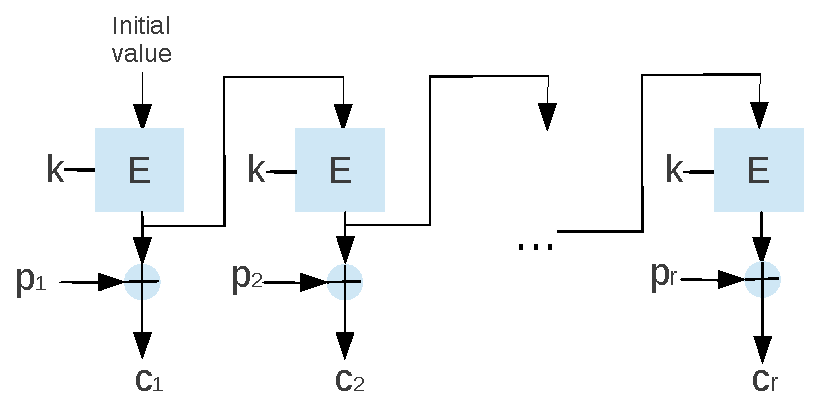
\includegraphics[scale=0.8]{./images/OFB_En}
\caption{Workflow of the OFB encryption. Adapted from
  \cite{DBLP:reference/crypt/2011}.}\label{OFBEN}
\end{figure}

\subsubsection*{Decryption}
Mathematical description : $P_i=C_i\oplus K_i\,,\,
K_i=E_K(K_{i-1})$.

The algorithm encryption is used in decryption as shown in Figure
\ref{OFBDE}. The keystream block $K_0$ is initialized with the start
value $IV$ or reinitialized by \texttt{Set\_IV()}. $K_{i-1}$ will be
encrypted to $K_i$ and XORed with $C_i$. The result of the operation
is the plaintext block $P_i$. These ciphertext blocks are decrypted in
the same sequence in which they are generated.
\begin{figure}[h]
\centering
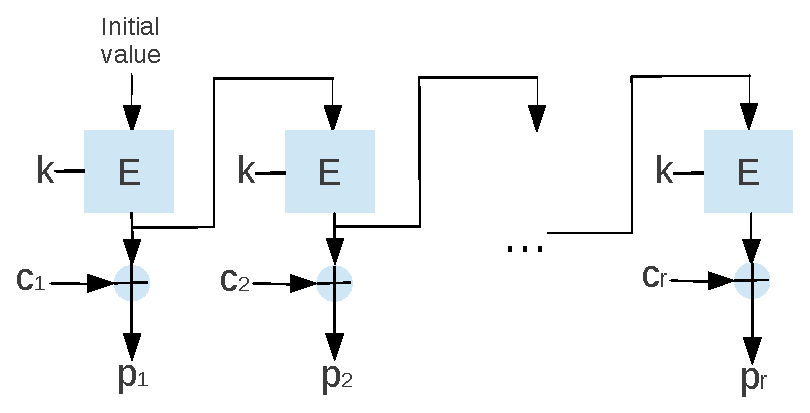
\includegraphics[scale=0.8]{./images/OFB_De}
\caption{Workflow of the OFB decryption. Adapted from
  \cite{DBLP:reference/crypt/2011}.}\label{OFBDE}
\end{figure}

\noindent\textbf{Remarks.}
With the "Low-Level-API" (\ref{Low-Level-OFB}) users can generate a
keystream without plaintext blocks. Thereby they can encrypt the
plaintext blocks very fast. For example it will be possible to
generate keystream blocks at night and then encrypt plaintext blocks
in the day time. So this mode is very suitable when phasic plaintext
blocks should be encrypted quickly.

\noindent\textbf{Notice.}
\begin{itemize}
\item The keystream repeats at any time. That is, $\exists
  L:K_0=K_L$. Supposed $m$ is the block size in bits, then the average
  length of a cycle goes to $2^m-1$ bits.
\item A bit error in plaintext will influence one bit in ciphertext
  and vice versa.
\item Manipulation on plaintext is clear, every change in ciphertext
  influences directly the plaintext.
\item Error in synchronization (Alice and Bob are in different counter
  states) can not be solved.
\end{itemize}

\subsubsection*{Low-Level-API}\label{Low-Level-OFB}
The following API can be used only when you know what it does.
\begin{lstlisting}{}
  procedure Next_Block(Keystream : out Block);
\end{lstlisting}
Mathematical description : $K_i=E_K(K_{i-1})$.

During initialization the start value IV is stored as keystream block
$K_0$. Every time when the \texttt{Next\_Block()} procedure is called,
the keystream block $K_i$ will be encrypted to $K_{i+1}$ and resulted
as keystream.

%%%%%%%%%%%%%%%%%%%%%%%%%%%%%%%%%%%%%%%%%%%%%%%%%%%%%%%%%%%
%%%%%%%%%%%%%%%%%%%%%%%%%%%%%%%%%%%%%%%%%%%%%%%%%%%%%%%%%%%

\section{Example}
\subsubsection*{CBC Mode}
\begin{lstlisting}{}
  with Crypto.Types;
  with Ada.Text_IO;
  with Crypto.Symmetric.Blockcipher_Tripledes;
  with Crypto.Symmetric.Mode.CBC;
  procedure Example_CBC_Mode is
	 use Ada.Text_IO; use Crypto.Types;
    package TDES renames Crypto.Symmetric.Blockcipher_Tripledes;
    -- use TDES in secure CBC mode
    package TDES_CBC is new Crypto.Symmetric.Mode.CBC(TDES);
	 use TDES_CBC;
    Key: B_Block192 := (16#00#, 16#00#, 16#00#, 16#00#, 16#00#,
                        16#00#, 16#00#, 16#00#, 16#00#, 16#00#,
                        16#00#, 16#00#, 16#00#, 16#00#, 16#00#,
                        16#00#, 16#01#, 16#23#, 16#45#, 16#67#,
                        16#89#, 16#ab#, 16#cd#, 16#ef#);
    IV: B_Block64 := (16#12#, 16#34#, 16#56#, 16#78#,
            	          16#90#, 16#ab#, 16#cd#, 16#ef#);
    --Plaintext
    P_String: String :="Now is the time for all.";
    P: array(1..3) of B_Block64 :=
			(To_B_Block64(To_Bytes(P_String(1..8))),
          To_B_Block64(To_Bytes(P_String(9..16))),
			 To_B_Block64(To_Bytes(P_String(17..24))));
    --Ciphertext
    C: array(0..3) of B_Block64;
    begin
      Init(Key, IV);    --1. Initialization
      C(0):= IV;        --1. Ciphertext block = start value
      for I in P'Range loop
	     Encrypt(P(I),C(I));  --Encryption
      end loop;
      --For decryption the start value will be
      --reinitialized with the same value.
      Set_IV(C(0));
      for I in P'Range loop
         Decrypt(C(I),P(I));   --Decryption
         Put(To_String(To_Bytes(P(I))));
      end loop;
  end Example_CBC_Mode;
\end{lstlisting}

\subsubsection*{BPS Mode}
\begin{lstlisting}{}
  with Crypto.Symmetric.Mode.BPS;
  with Crypto.Symmetric.Blockcipher_AES128;
  with Crypto.Types; use Crypto.Types;
  with Ada.Text_IO; use Ada.Text_IO;
  procedure Example_BPS_Mode is
    package AES128 renames Crypto.Symmetric.Blockcipher_AES128;
    package BPS is new Crypto.Symmetric.Mode.BPS(AES128);
    use BPS;
    Key : B_Block128 := (16#12#, 16#34#, 16#56#, 16#78#,
	  	                 16#90#, 16#ab#, 16#cd#, 16#ef#,
		                 16#12#, 16#34#, 16#56#, 16#78#,
		                 16#90#, 16#ab#, 16#cd#, 16#ef#);
    IV : B_Block64 :=(16#12#, 16#34#, 16#56#, 16#78#,
		                16#90#, 16#ab#, 16#cd#, 16#ef#);
    Plaintext : BPS.Numerals(1..10) := (0,1,2,3,4,5,6,7,8,9);
    Ciphertext, P : BPS.Numerals(1..10);
    Result : Boolean := False;
  begin
    Init(Key, IV);
    Encrypt(Plaintext, Ciphertext);
    Decrypt(Ciphertext, P);
    for I in Plaintext'Range loop
       if Plaintext(I) = P(I) then
          Result := True;
       end if;
    end loop;
    if Result then
       Put_Line("OK");
    else
       Put_Line("Error");
    end if;
  end Example_BPS_Mode;
\end{lstlisting}
